\section{Pierwsze poprawki}

W celu wprowadzenia większej różnorodności w systemie wprowadzone zostały zmiany. Każdy agent uzyskał współczynnik daru przekonywania $A_i$, który pozwoli na zróżnicowanie wpływu agentów.
% 1a. Huby mają większy dar przekonywania
Ponadto huby powinny mieć większy dar przekonywania. W celu uzyskania takiego efektu należało zwiększyć siłę oddziaływania węzłów z dużą liczbą sąsiadów.
% 1b. Dar przekonywania nie zależy od rangi (stopnia) wierzchołka
% Dar przekonywania nie powinien zależeć od stopnia wierzchołka, ponieważ nie są to wielkości skorelowane.
% 1c. Konserwatyzm osobnika
Ponadto każdy agent powinien mieć właściwość zwaną elastycznością, która zwiększa prawdopodobieństwo, że dany agent zmieni swoją opinię.
% 2. Wyliczyliśmy średnią pozycję sąsiadów:
% 2a Gdzie i z jakim prawdopodobieństwem może przesunąć się osobnik?
% 2b. Jak zapisać zmianę energii związaną z potencjalną zmianą miejsca w przestrzeni rozwiązań?
% 2c. Z małym prawdopodobieństwem (wsp. konserwatyzmu) osobnik godzi się zmienić swoją opinię
% 2d. Załóżmy, że istnieje parametr \beta na poziomie 0.1, takie, że zmianę pozycji osobnika losujemy na prostej od jego aktualnej pozycji do położenia średniego.
%     Losujemy z rozkładu wykładniczego o średniej \beta*odległość(obiekt, średnia sąsiadów)
Zaszła również potrzeba zmiany rozkładu, z którego była losowana nowa opinia agenta, ponieważ poprzedni rozkład trójkątny powodował szybkie zbieganie opinii do jednego centrum.
Wybór padł na rozkład wykładniczy.

\begin{figure}
    \centering
    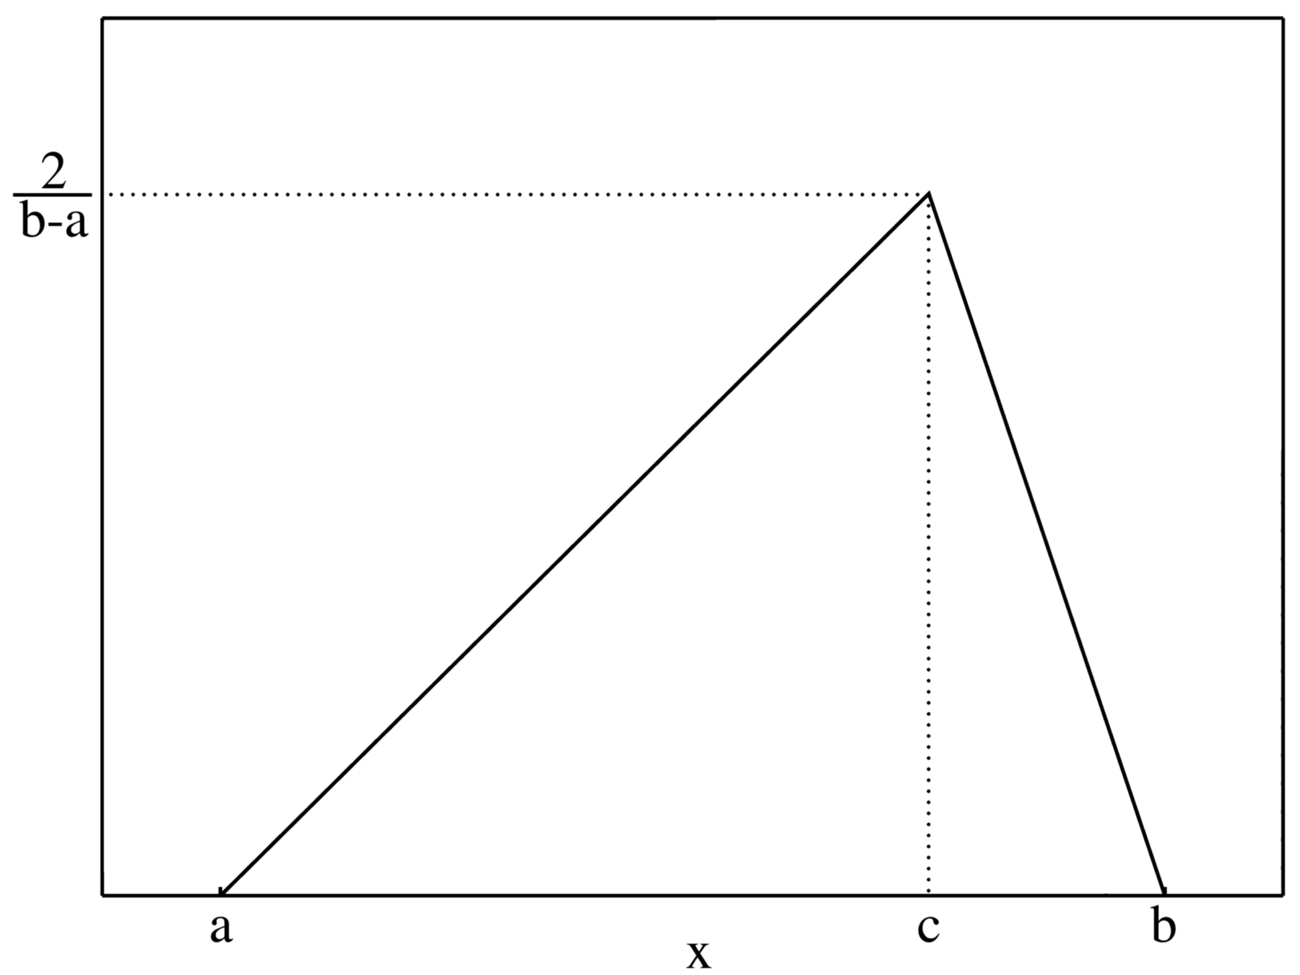
\includegraphics[width=0.5\textwidth]{img/Triangular_distribution_PMF.png}
    \caption{Rozkład trójkątny. Źródło: \cite{rozklad_trojkatny_wykres}}
    \label{fig:rozklad_trojkatny}
\end{figure}
\begin{figure}
    \centering
    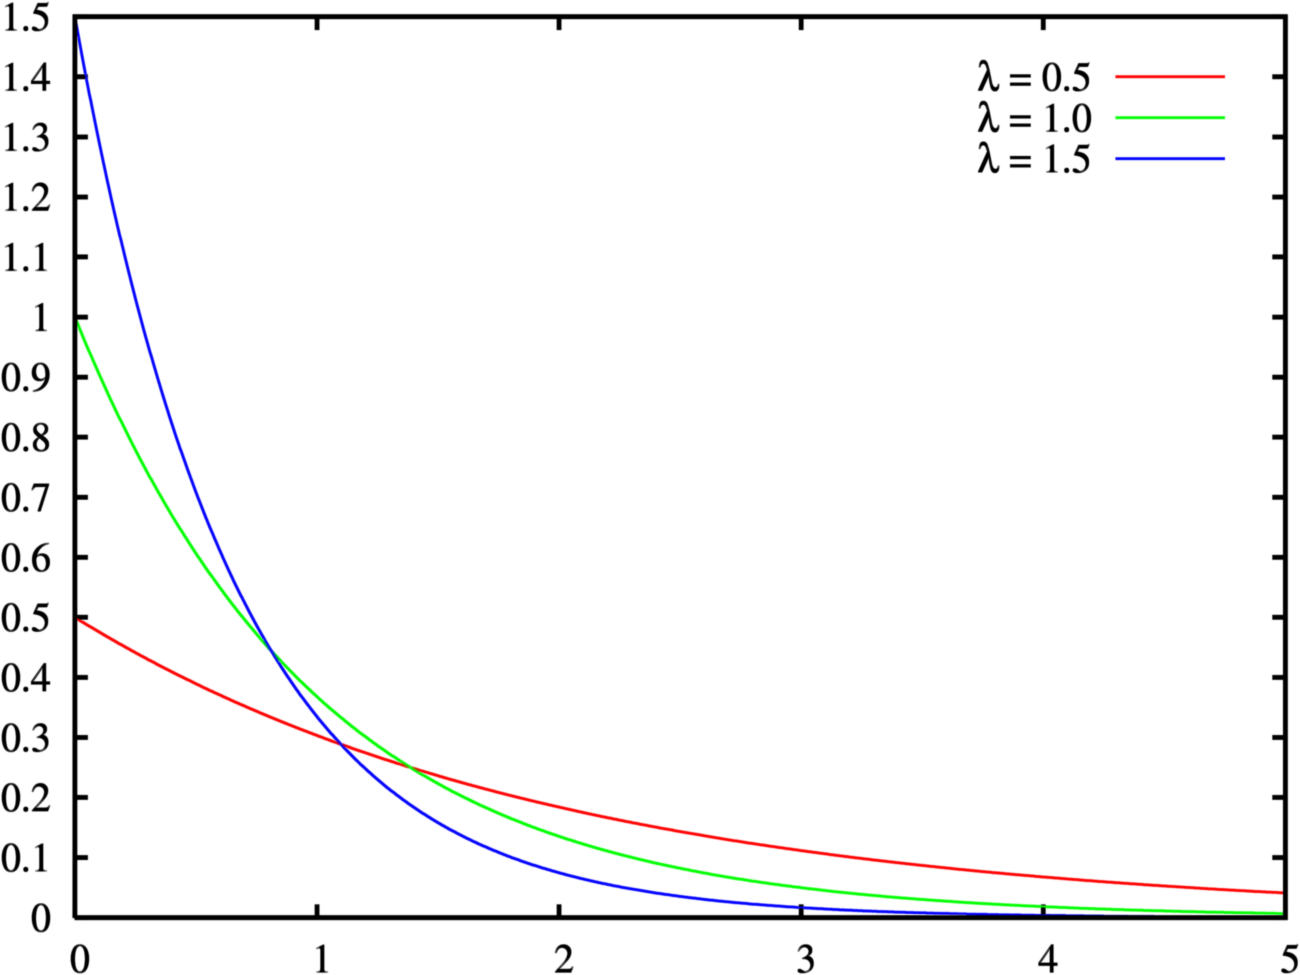
\includegraphics[width=0.5\textwidth]{img/Exponential_distribution_pdf.png}
    \caption{Rozkład wykładniczy. Źródło: \cite{rozklad_wykladniczy_wykres}}
    \label{fig:rozklad_wykladniczy}
\end{figure}

\newpage

\subsection{Zmieniona implementacja}

Na nowo zaimplementowany agent ma trzy własności — opinię, elastyczność zmiany opinii i wpływ na innych.
Opinia agenta na początku jest losowana z rozkładu równomiernego, podobnie jak wpływ na innych.
Elastyczność z kolei jest losowana z rozkładu beta tak, żeby była względnie mała.
Opinie są aktualizowane, bazując na rozkładzie trójkątnym oraz własnościach agenta i jego sąsiadów.
Wyliczana jest średnia opinia sąsiadów oraz średnia ich wpływu.
Następnie obliczany jest udział sąsiadów agenta w ogólnej liczbie węzłów, który bierze udział w przesuwaniu środka rozkładu.
Przesunięcie obliczane jest wg wzoru:
przesunięcie = elastyczność agenta * (udział sąsiadów agenta w populacji + wpływ sąsiadów)

Sumowanie wpływu sąsiadów z udziałem sąsiadów agenta w populacji powoduje, że na agenta z większą ilością sąsiadów wywierany jest większy wpływ.
Z drugiej strony, na odizolowanych osobników wywierany jest mniejszy wpływ, co powoduje, że 'okopują' się oni w swoich poglądach.
Z kolei elastyczność agenta we wzorze pozwala ograniczyć wpływ otoczenia na danego agenta.

Rezultat jest taki, że huby mają duży wpływ na bliskie poglądowo węzły, zacieśniając je coraz bardziej, natomiast węzły z małą liczbą sąsiadów przesuwają się w kierunku huba dużo wolniej.